% Created by tikzDevice version 0.6.2 on 2012-09-11 12:28:03
% !TEX encoding = UTF-8 Unicode
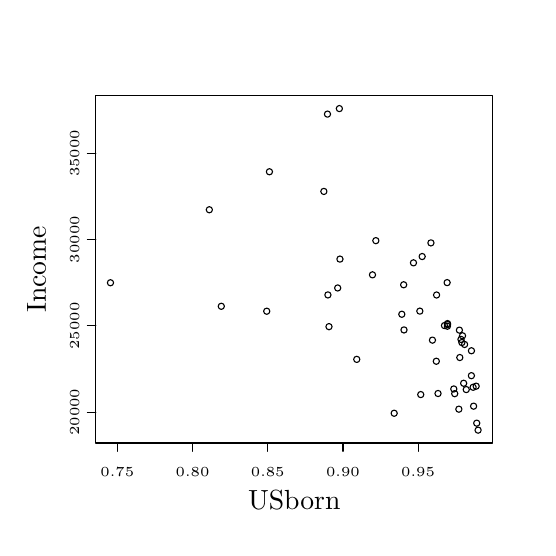
\begin{tikzpicture}[x=1pt,y=1pt,scale=0.5]
\definecolor[named]{drawColor}{rgb}{0.00,0.00,0.00}
\definecolor[named]{fillColor}{rgb}{1.00,1.00,1.00}
\fill[color=fillColor,fill opacity=0.00,] (0,0) rectangle (361.35,361.35);
\begin{scope}
\path[clip] ( 49.20, 61.20) rectangle (336.15,312.15);
\definecolor[named]{fillColor}{rgb}{0.00,0.00,0.00}
\definecolor[named]{drawColor}{rgb}{0.00,0.00,0.00}

\draw[color=drawColor,line cap=round,line join=round,fill opacity=0.00,] (321.92,101.46) circle (  2.25);

\draw[color=drawColor,line cap=round,line join=round,fill opacity=0.00,] (270.39,154.23) circle (  2.25);

\draw[color=drawColor,line cap=round,line join=round,fill opacity=0.00,] (237.82,121.63) circle (  2.25);

\draw[color=drawColor,line cap=round,line join=round,fill opacity=0.00,] (322.27, 87.80) circle (  2.25);

\draw[color=drawColor,line cap=round,line join=round,fill opacity=0.00,] ( 59.83,177.01) circle (  2.25);

\draw[color=drawColor,line cap=round,line join=round,fill opacity=0.00,] (278.80,191.40) circle (  2.25);

\draw[color=drawColor,line cap=round,line join=round,fill opacity=0.00,] (225.25,302.86) circle (  2.25);

\draw[color=drawColor,line cap=round,line join=round,fill opacity=0.00,] (291.43,205.82) circle (  2.25);

\draw[color=drawColor,line cap=round,line join=round,fill opacity=0.00,] (216.67,298.87) circle (  2.25);

\draw[color=drawColor,line cap=round,line join=round,fill opacity=0.00,] (172.76,156.43) circle (  2.25);

\draw[color=drawColor,line cap=round,line join=round,fill opacity=0.00,] (301.22,146.06) circle (  2.25);

\draw[color=drawColor,line cap=round,line join=round,fill opacity=0.00,] (139.93,159.99) circle (  2.25);

\draw[color=drawColor,line cap=round,line join=round,fill opacity=0.00,] (296.56, 96.96) circle (  2.25);

\draw[color=drawColor,line cap=round,line join=round,fill opacity=0.00,] (225.68,194.09) circle (  2.25);

\draw[color=drawColor,line cap=round,line join=round,fill opacity=0.00,] (313.14,136.08) circle (  2.25);

\draw[color=drawColor,line cap=round,line join=round,fill opacity=0.00,] (315.76,132.41) circle (  2.25);

\draw[color=drawColor,line cap=round,line join=round,fill opacity=0.00,] (303.32,145.58) circle (  2.25);

\draw[color=drawColor,line cap=round,line join=round,fill opacity=0.00,] (324.10,102.26) circle (  2.25);

\draw[color=drawColor,line cap=round,line join=round,fill opacity=0.00,] (307.96,100.26) circle (  2.25);

\draw[color=drawColor,line cap=round,line join=round,fill opacity=0.00,] (295.32,120.28) circle (  2.25);

\draw[color=drawColor,line cap=round,line join=round,fill opacity=0.00,] (251.62,207.43) circle (  2.25);

\draw[color=drawColor,line cap=round,line join=round,fill opacity=0.00,] (214.06,243.01) circle (  2.25);

\draw[color=drawColor,line cap=round,line join=round,fill opacity=0.00,] (283.42,156.50) circle (  2.25);

\draw[color=drawColor,line cap=round,line join=round,fill opacity=0.00,] (303.14,177.10) circle (  2.25);

\draw[color=drawColor,line cap=round,line join=round,fill opacity=0.00,] (325.52, 70.49) circle (  2.25);

\draw[color=drawColor,line cap=round,line join=round,fill opacity=0.00,] (314.27,138.67) circle (  2.25);

\draw[color=drawColor,line cap=round,line join=round,fill opacity=0.00,] (311.62, 85.63) circle (  2.25);

\draw[color=drawColor,line cap=round,line join=round,fill opacity=0.00,] (312.00,142.75) circle (  2.25);

\draw[color=drawColor,line cap=round,line join=round,fill opacity=0.00,] (224.04,173.24) circle (  2.25);

\draw[color=drawColor,line cap=round,line join=round,fill opacity=0.00,] (285.10,195.95) circle (  2.25);

\draw[color=drawColor,line cap=round,line join=round,fill opacity=0.00,] (174.71,257.22) circle (  2.25);

\draw[color=drawColor,line cap=round,line join=round,fill opacity=0.00,] (264.86, 82.69) circle (  2.25);

\draw[color=drawColor,line cap=round,line join=round,fill opacity=0.00,] (131.29,229.76) circle (  2.25);

\draw[color=drawColor,line cap=round,line join=round,fill opacity=0.00,] (313.79,133.80) circle (  2.25);

\draw[color=drawColor,line cap=round,line join=round,fill opacity=0.00,] (315.08,104.36) circle (  2.25);

\draw[color=drawColor,line cap=round,line join=round,fill opacity=0.00,] (303.42,147.48) circle (  2.25);

\draw[color=drawColor,line cap=round,line join=round,fill opacity=0.00,] (308.62, 96.85) circle (  2.25);

\draw[color=drawColor,line cap=round,line join=round,fill opacity=0.00,] (271.97,142.90) circle (  2.25);

\draw[color=drawColor,line cap=round,line join=round,fill opacity=0.00,] (295.52,168.15) circle (  2.25);

\draw[color=drawColor,line cap=round,line join=round,fill opacity=0.00,] (216.98,168.21) circle (  2.25);

\draw[color=drawColor,line cap=round,line join=round,fill opacity=0.00,] (316.94, 99.80) circle (  2.25);

\draw[color=drawColor,line cap=round,line join=round,fill opacity=0.00,] (320.67,109.84) circle (  2.25);

\draw[color=drawColor,line cap=round,line join=round,fill opacity=0.00,] (320.71,127.85) circle (  2.25);

\draw[color=drawColor,line cap=round,line join=round,fill opacity=0.00,] (217.76,145.28) circle (  2.25);

\draw[color=drawColor,line cap=round,line join=round,fill opacity=0.00,] (284.06, 96.19) circle (  2.25);

\draw[color=drawColor,line cap=round,line join=round,fill opacity=0.00,] (292.53,135.53) circle (  2.25);

\draw[color=drawColor,line cap=round,line join=round,fill opacity=0.00,] (271.72,175.54) circle (  2.25);

\draw[color=drawColor,line cap=round,line join=round,fill opacity=0.00,] (249.19,182.72) circle (  2.25);

\draw[color=drawColor,line cap=round,line join=round,fill opacity=0.00,] (324.52, 75.53) circle (  2.25);

\draw[color=drawColor,line cap=round,line join=round,fill opacity=0.00,] (303.47,146.80) circle (  2.25);

\draw[color=drawColor,line cap=round,line join=round,fill opacity=0.00,] (312.30,122.96) circle (  2.25);
\end{scope}
\begin{scope}
\path[clip] (  0.00,  0.00) rectangle (361.35,361.35);
\definecolor[named]{fillColor}{rgb}{0.00,0.00,0.00}
\definecolor[named]{drawColor}{rgb}{0.00,0.00,0.00}

\draw[color=drawColor,line cap=round,line join=round,fill opacity=0.00,] ( 64.82, 61.20) -- (282.19, 61.20);

\draw[color=drawColor,line cap=round,line join=round,fill opacity=0.00,] ( 64.82, 61.20) -- ( 64.82, 55.20);

\draw[color=drawColor,line cap=round,line join=round,fill opacity=0.00,] (119.16, 61.20) -- (119.16, 55.20);

\draw[color=drawColor,line cap=round,line join=round,fill opacity=0.00,] (173.50, 61.20) -- (173.50, 55.20);

\draw[color=drawColor,line cap=round,line join=round,fill opacity=0.00,] (227.85, 61.20) -- (227.85, 55.20);

\draw[color=drawColor,line cap=round,line join=round,fill opacity=0.00,] (282.19, 61.20) -- (282.19, 55.20);

\node[color=drawColor,anchor=base,inner sep=0pt, outer sep=0pt, scale=  1.00] at ( 64.82, 37.20) {\tiny 0.75};
\node[color=drawColor,anchor=base,inner sep=0pt, outer sep=0pt, scale=  1.00] at (119.16, 37.20) {\tiny 0.80};
\node[color=drawColor,anchor=base,inner sep=0pt, outer sep=0pt, scale=  1.00] at (173.50, 37.20) {\tiny 0.85};
\node[color=drawColor,anchor=base,inner sep=0pt, outer sep=0pt, scale=  1.00] at (227.85, 37.20) {\tiny 0.90};
\node[color=drawColor,anchor=base,inner sep=0pt, outer sep=0pt, scale=  1.00] at (282.19, 37.20) {\tiny 0.95};

\draw[color=drawColor,line cap=round,line join=round,fill opacity=0.00,] ( 49.20, 83.48) -- ( 49.20,270.47);

\draw[color=drawColor,line cap=round,line join=round,fill opacity=0.00,] ( 49.20, 83.48) -- ( 43.20, 83.48);

\draw[color=drawColor,line cap=round,line join=round,fill opacity=0.00,] ( 49.20,145.81) -- ( 43.20,145.81);

\draw[color=drawColor,line cap=round,line join=round,fill opacity=0.00,] ( 49.20,208.14) -- ( 43.20,208.14);

\draw[color=drawColor,line cap=round,line join=round,fill opacity=0.00,] ( 49.20,270.47) -- ( 43.20,270.47);

\node[rotate= 90.00,color=drawColor,anchor=base,inner sep=0pt, outer sep=0pt,
scale=  1.00] at ( 37.20, 83.48) {\tiny 20000};

\node[rotate= 90.00,color=drawColor,anchor=base,inner sep=0pt, outer sep=0pt,
scale=  1.00] at ( 37.20,145.81) {\tiny 25000};

\node[rotate= 90.00,color=drawColor,anchor=base,inner sep=0pt, outer sep=0pt,
scale=  1.00] at ( 37.20,208.14) {\tiny 30000};

\node[rotate= 90.00,color=drawColor,anchor=base,inner sep=0pt, outer sep=0pt,
scale=  1.00] at ( 37.20,270.47) {\tiny 35000};

\draw[color=drawColor,line cap=round,line join=round,fill opacity=0.00,] ( 49.20, 61.20) --
	(336.15, 61.20) --
	(336.15,312.15) --
	( 49.20,312.15) --
	( 49.20, 61.20);
\end{scope}
\begin{scope}
\path[clip] (  0.00,  0.00) rectangle (361.35,361.35);
\definecolor[named]{fillColor}{rgb}{0.00,0.00,0.00}
\definecolor[named]{drawColor}{rgb}{0.00,0.00,0.00}

\node[color=drawColor,anchor=base,inner sep=0pt, outer sep=0pt, scale=  1.00]
at (192.67, 13.20) {USborn};

\node[rotate= 90.00,color=drawColor,anchor=base,inner sep=0pt, outer sep=0pt,
scale=  1.00] at ( 13.20,186.67) {Income};
\end{scope}
\end{tikzpicture}
